\subsection{Optimization Results}\label{sec:optimization_results}
In this section, we present and analyze the results of running the Optimization experiment that we described in Section~\ref{subsec:optimization_experiment_design}.
As mentioned, our primary objective was to identify the optimal configurations for predicting the concentration of various oxides in our dataset.
We systematically evaluated a range of machine learning models, preprocessing techniques, and hyperparameter settings to determine the most effective combinations for each oxide.

The results of the experiment were ~$16.000$ trials worth of data on the configurations used, hyperparameters, as well as metrics.

Our data cleaning for this dataset primarily included filtering out failed runs, which was caused by configurations that did not work well together, as well as filtering out extreme error values.
We filter out any runs that had a \gls{rmsecv} above 50.
Approaches like \gls{svr} could occasionally yield this kind of outlier result in specific configurations.
We selected 50 as threshold to include as many trials that were not obvious outliers.

Our experiment underwent mostly without issues.
Some issues are to be expected given the scale of the experiment.
Unfortunately, we encountered an issue with a server we were using, resulting in some oxides and models having to be re-run.
We managed to recover and re-run most of these.
However, \gls{ngboost} for \ce{MgO} was only partially finished.
Given that each model of the ten models would undergo 200 trials, for each oxide, this resulted in 2000 runs per oxide.
The exception is \ce{MgO}, for which \gls{ngboost} ran 143 trials, making the total trials for \ce{MgO} 1943.
After the filtering process, we are left with a total of 15245 trials to analyze.

Given that we stored the configurations as well as each hyperparameter value for the trials, we had \~100 variables to consider during our analysis.
Of these, the primary variables of interest are the metrics, as well as overall configuration variables, namely \texttt{Model Type}, \texttt{Scaler Type}, \texttt{PCA Type}, \texttt{Transformer Type}.

As we described in Section~\ref{sec:optimization_framework}, our optimization system searches for the best configurations by through multi-objective optimization.
The optimization process is facilitated by adjusting the configuration and hyperparameters of the machine learning model and preprocessing pipeline, therefore minimizing the objective.
Because the sampler will do initial exploration, and then attempt to find the optimal configuration through exploitation, we'll see that the values of variables that frequently appear in the results are the ones that are most likely to be optimal.
Looking at the results in tables \ref{tab:scalers_comparison}, \ref{tab:pca_comparison}, and \ref{tab:transformers_comparison}, we can see these values for the various preprocessors.
The optimization results show that the configurations with the highest total values across oxides are indicative of being the most frequently exploited, hence most likely to optimize performance. 
\texttt{Norm3Scaler} was used in 5090 trials, and therefore appears to be the most effective scaler.
This was somewhat expected, given the method was created for this particular type of \gls{libs} dataset, as discussed in Section~\ref{sec:norm3}.
For dimensionality reduction, we see that \texttt{None}, indicating no \gls{pca}, was used in 9419 trials, which is \~59\% of all trials.
This suggests that either no dimensionality reduction is optimal, or a better method should be identified.
Neither \gls{pca} nor \gls{kernel-pca} are very effective for this dataset.
\texttt{QuantileTransformer} was used in 5710 trials, and therefore seems to be the most optimal transformer.
We note that \texttt{PowerTransformer} was used in 5277 trials, with and no transformer in 4956. As opposed to the other preprocessing method types, there does not seem to be a clear winner for the transformers.

\begin{table*}
    \centering
    \begin{tabular}{lccccccccc}
        \toprule
        \textbf{Oxide} & \texttt{MaxAbsScaler} & \texttt{MinMaxScaler} & \texttt{Norm3Scaler} & \texttt{RobustScaler} & \texttt{StandardScaler} \\
        \midrule
        \ce{Al2O3}               & 336  & 476  & 495  & 453  & 240 \\
        \ce{CaO}                 & 310  & 362  & 681  & 338  & 309 \\
        \ce{FeO_T}               & 498  & 287  & 561  & 339  & 315 \\
        \ce{K2O}                 & 258  & 320  & 622  & 430  & 370 \\
        \ce{MgO}                 & 239  & 340  & 646  & 413  & 305 \\
        \ce{Na2O}                & 316  & 327  & 748  & 320  & 289 \\
        \ce{SiO2}                & 221  & 421  & 830  & 309  & 219 \\
        \ce{TiO2}                & 280  & 322  & 507  & 565  & 326 \\
        Total across oxides      & 2458 & 2855 & 5090 & 3167 & 2373 \\
        \bottomrule
    \end{tabular}
    \caption{Comparison of different scalers across the eight major oxides.}
    \label{tab:scalers_comparison}
\end{table*}


\begin{table*}
    \centering
    \begin{tabular}{lccccccccc}
        \toprule
        \textbf{Oxide} & \texttt{None} & \texttt{KernelPCA} & \texttt{PCA} \\
        \midrule
        \ce{Al2O3}               & 1243  & 389  & 368 \\
        \ce{CaO}                 & 1246  & 374  & 380 \\
        \ce{FeO_T}               & 1217  & 382  & 401 \\
        \ce{K2O}                 & 1250  & 373  & 377 \\
        \ce{MgO}                 & 1037  & 543  & 363 \\
        \ce{Na2O}                & 1167  & 382  & 451 \\
        \ce{SiO2}                & 1096  & 457  & 447 \\
        \ce{TiO2}                & 1163  & 468  & 369 \\
        Total across oxides      & 9419  & 3368 & 3156 \\
        \bottomrule
    \end{tabular}
    \caption{Comparison of different PCA types across the eight major oxides.}
    \label{tab:pca_comparison}
\end{table*}


\begin{table*}
    \centering
    \begin{tabular}{lccccccccc}
        \toprule
        \textbf{Oxide} & \texttt{None} & \texttt{PowerTransformer} & \texttt{QuantileTransformer} \\
        \midrule
        \ce{Al2O3}               & 442  & 649  & 909 \\
        \ce{CaO}                 & 673  & 595  & 732 \\
        \ce{FeO_T}               & 633  & 644  & 723 \\
        \ce{K2O}                 & 504  & 822  & 674 \\
        \ce{MgO}                 & 725  & 701  & 517 \\
        \ce{Na2O}                & 441  & 583  & 976 \\
        \ce{SiO2}                & 760  & 566  & 674 \\
        \ce{TiO2}                & 778  & 717  & 505 \\
        Total across oxides      & 4956 & 5277 & 5710 \\
        \bottomrule
    \end{tabular}
    \caption{Comparison of different transformers across the eight major oxides.}
    \label{tab:transformers_comparison}
\end{table*}



\begin{figure*}
    \centering
    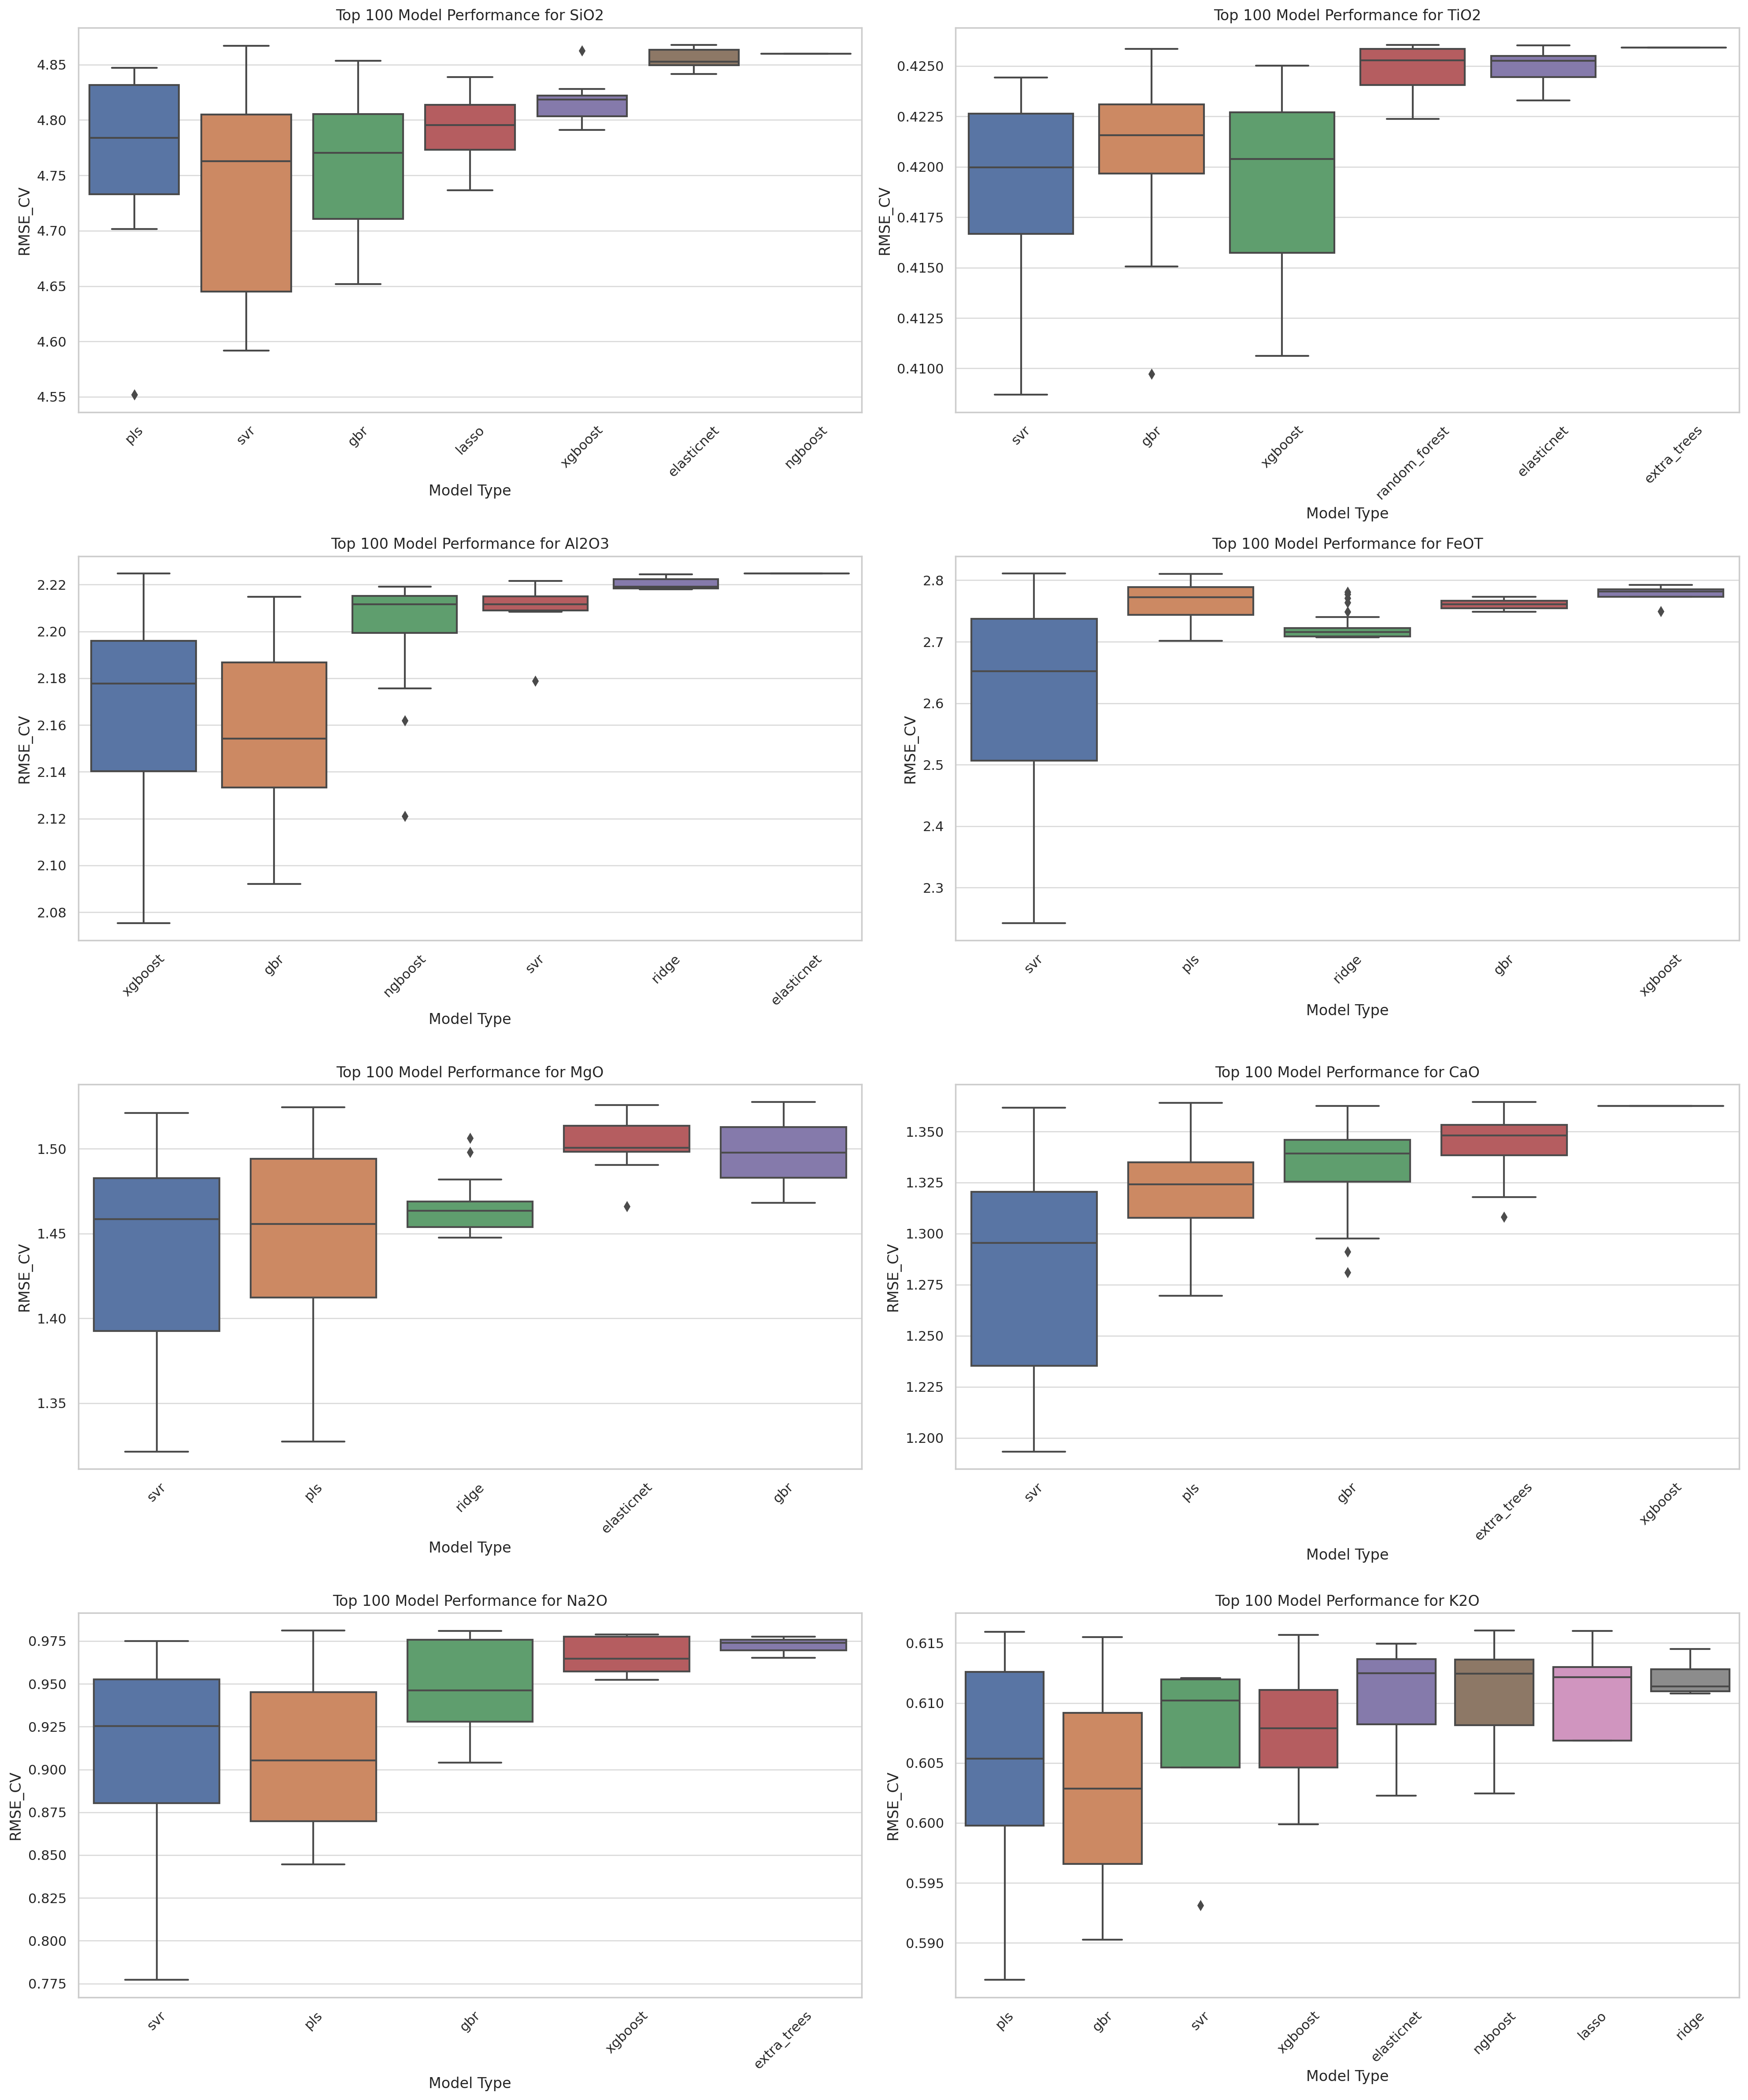
\includegraphics[width=\textwidth]{images/top100/models.png}
    \caption{Top 100 model performance across oxides. The subplots show the distribution of \gls{rmsecv} values for the top 100 trials for each model type across the eight different oxides. This helps identify the most effective models for each oxide within the top-performing trials.}
    \label{fig:top100_models}
\end{figure*}

\begin{figure*}
    \centering
    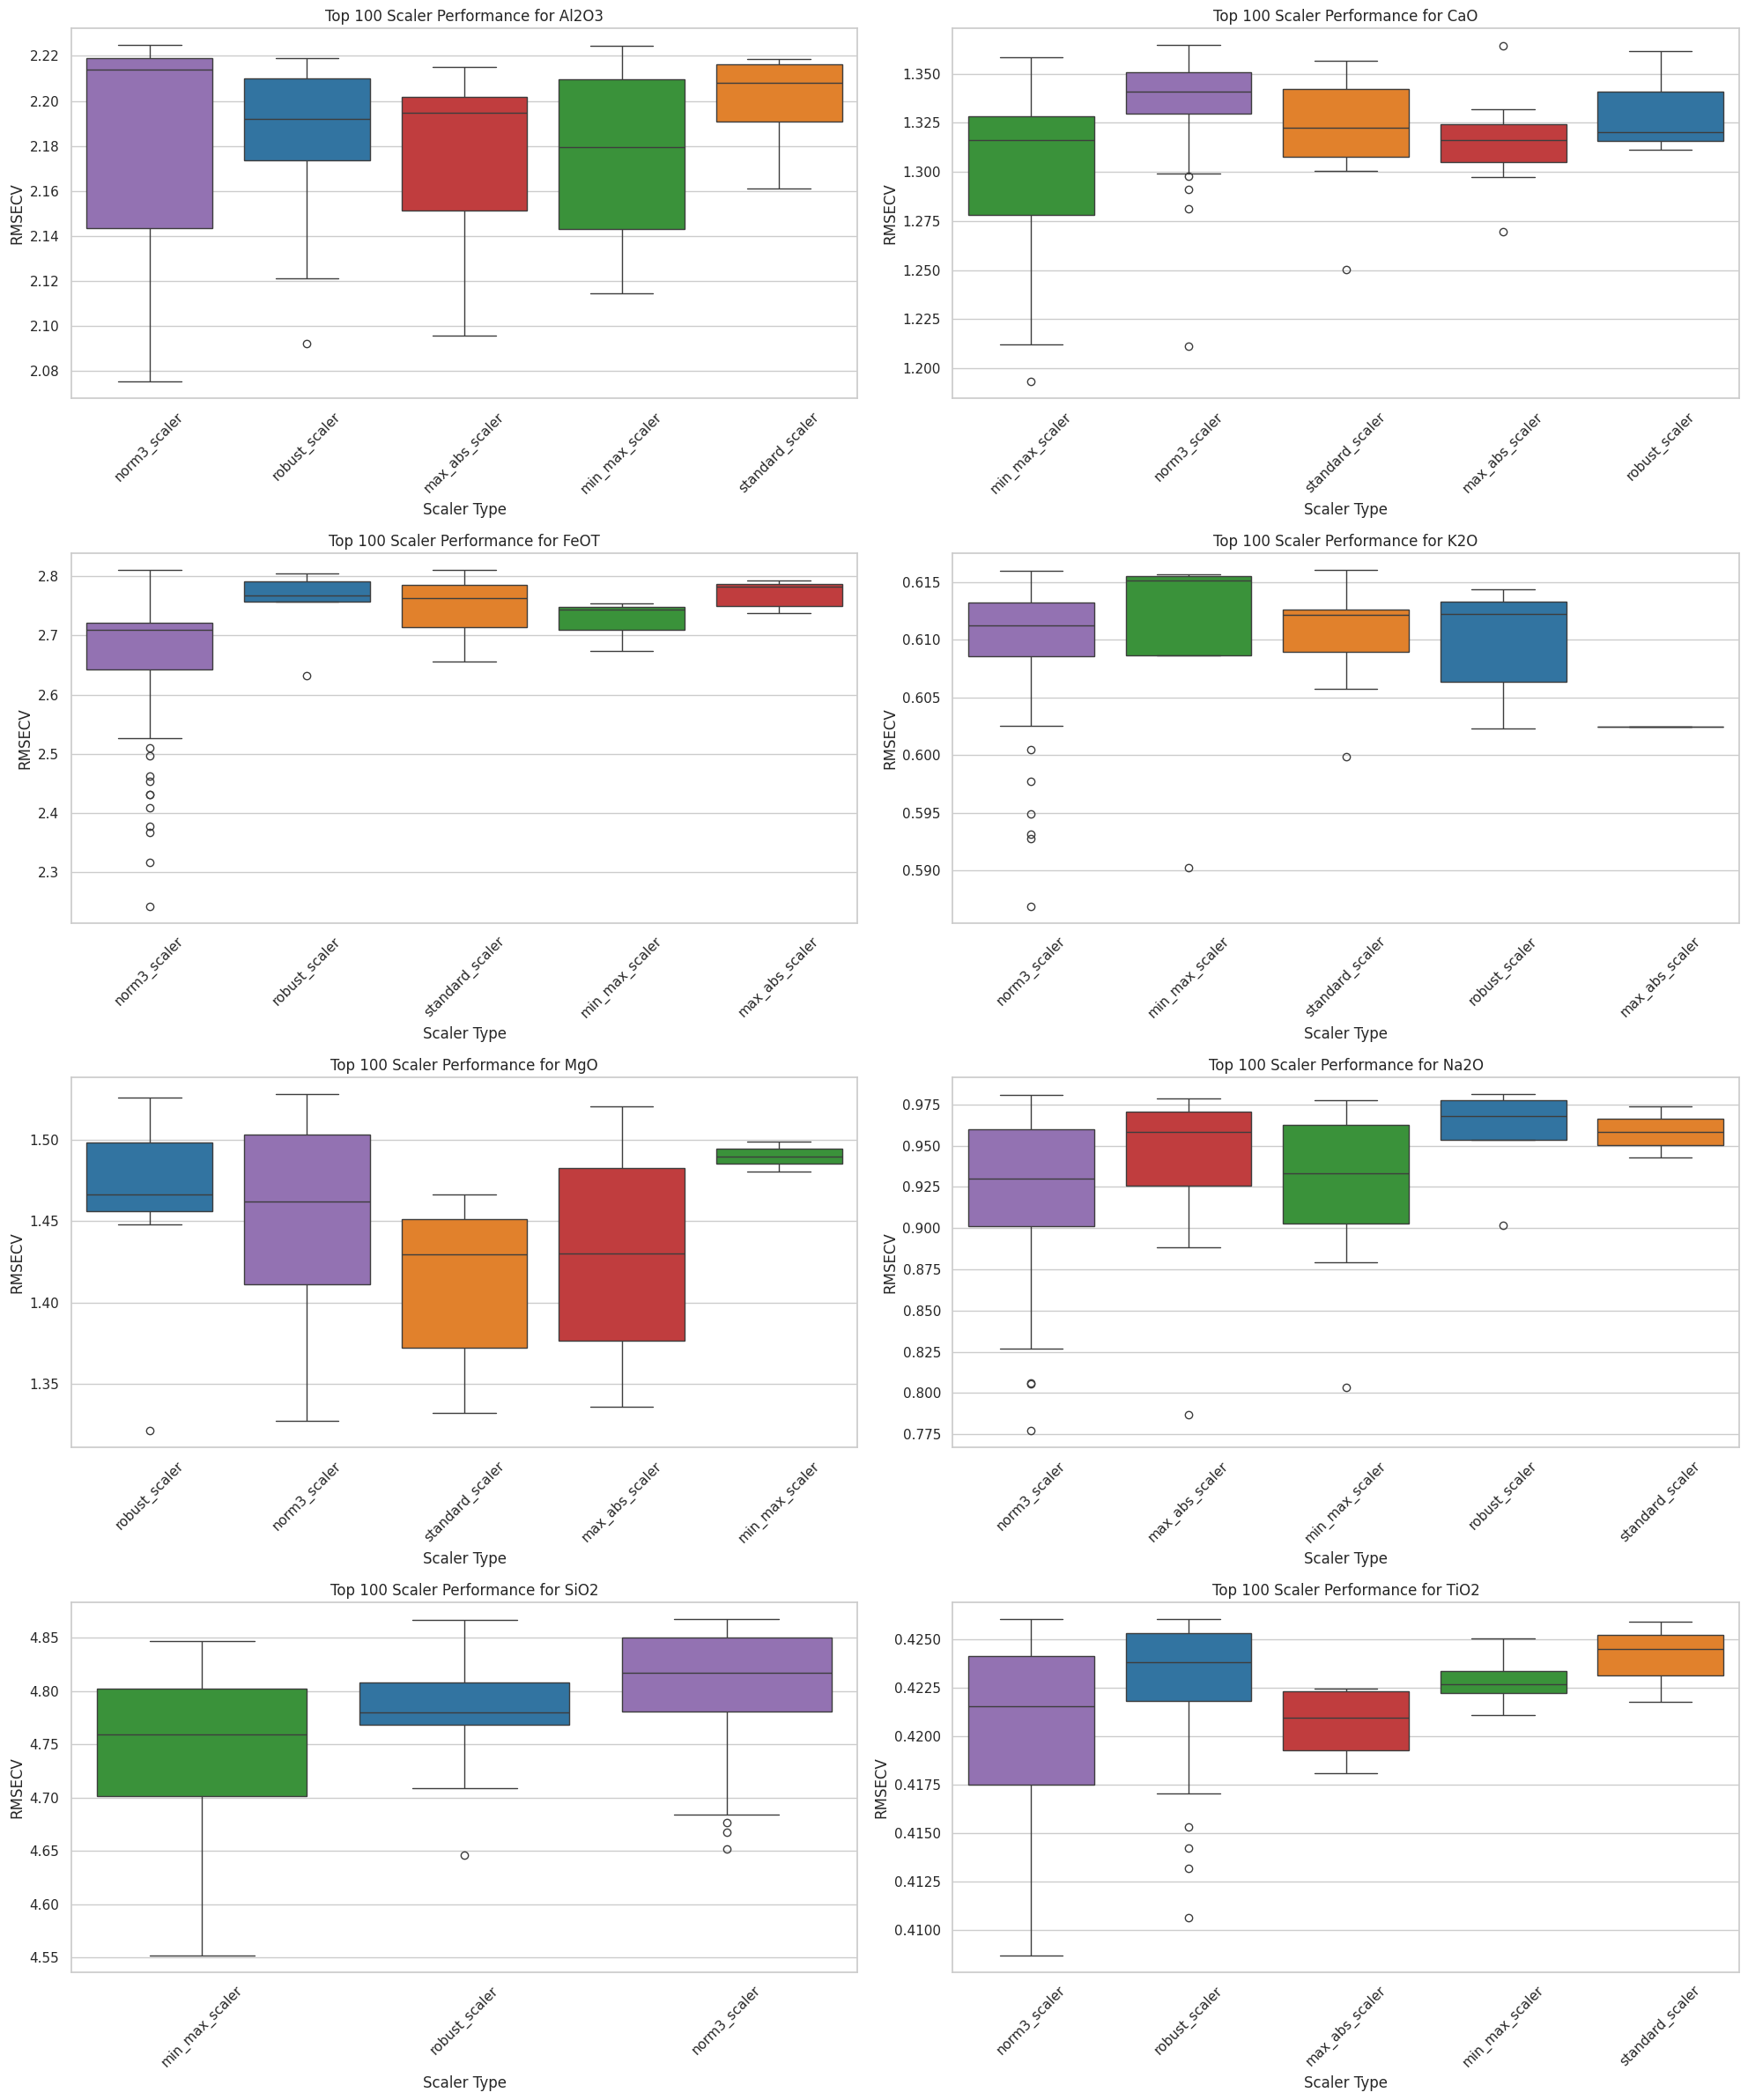
\includegraphics[width=\textwidth]{images/top100/scalers.png}
    \caption{Top 100 scaler performance across oxides. The subplots illustrate the distribution of \gls{rmsecv} values for the top 100 trials for each scaler type across the different oxides. This helps pinpoint which scalers perform best within the top-performing trials.}
    \label{fig:top100_scalers}
\end{figure*}

\begin{figure*}
    \centering
    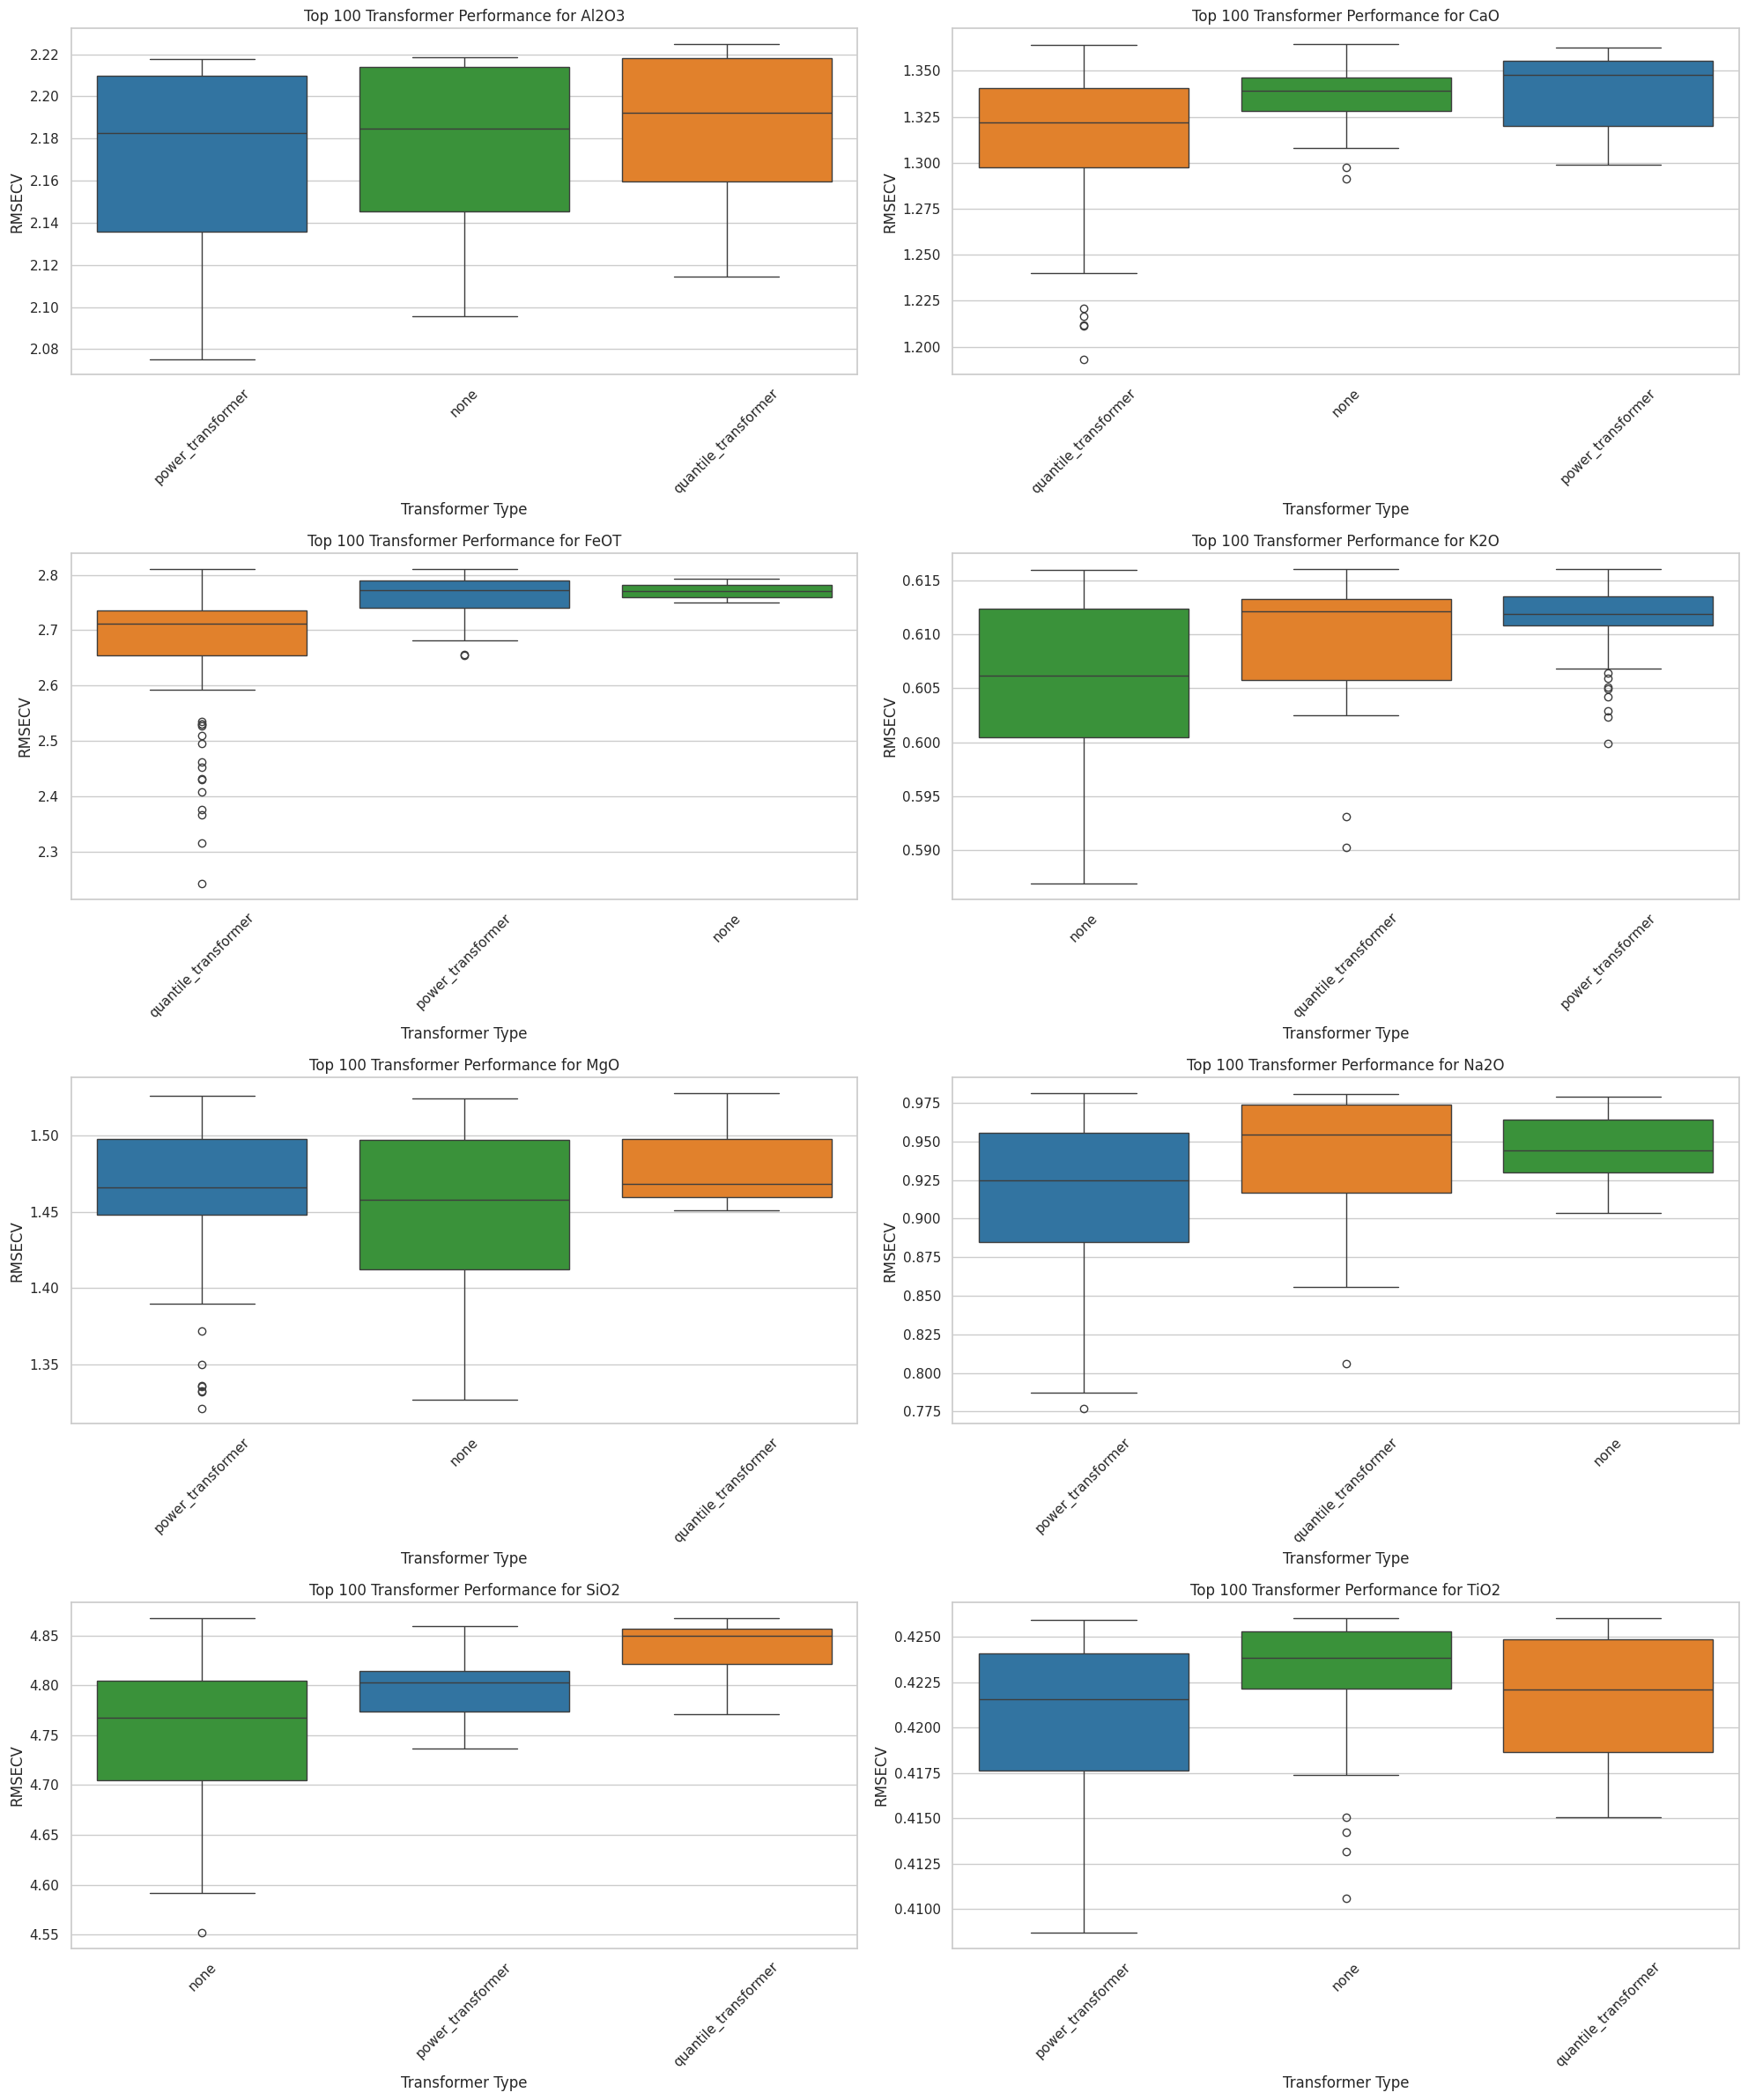
\includegraphics[width=\textwidth]{images/top100/transformers.png}
    \caption{Top 100 transformer performance across oxides. The subplots display the distribution of \gls{rmsecv} values for the top 100 trials for each transformer type across the different oxides. This helps determine the effectiveness of each transformer for different oxides within the top-performing trials.}
    \label{fig:top100_transformers}
\end{figure*}

\begin{figure*}
    \centering
    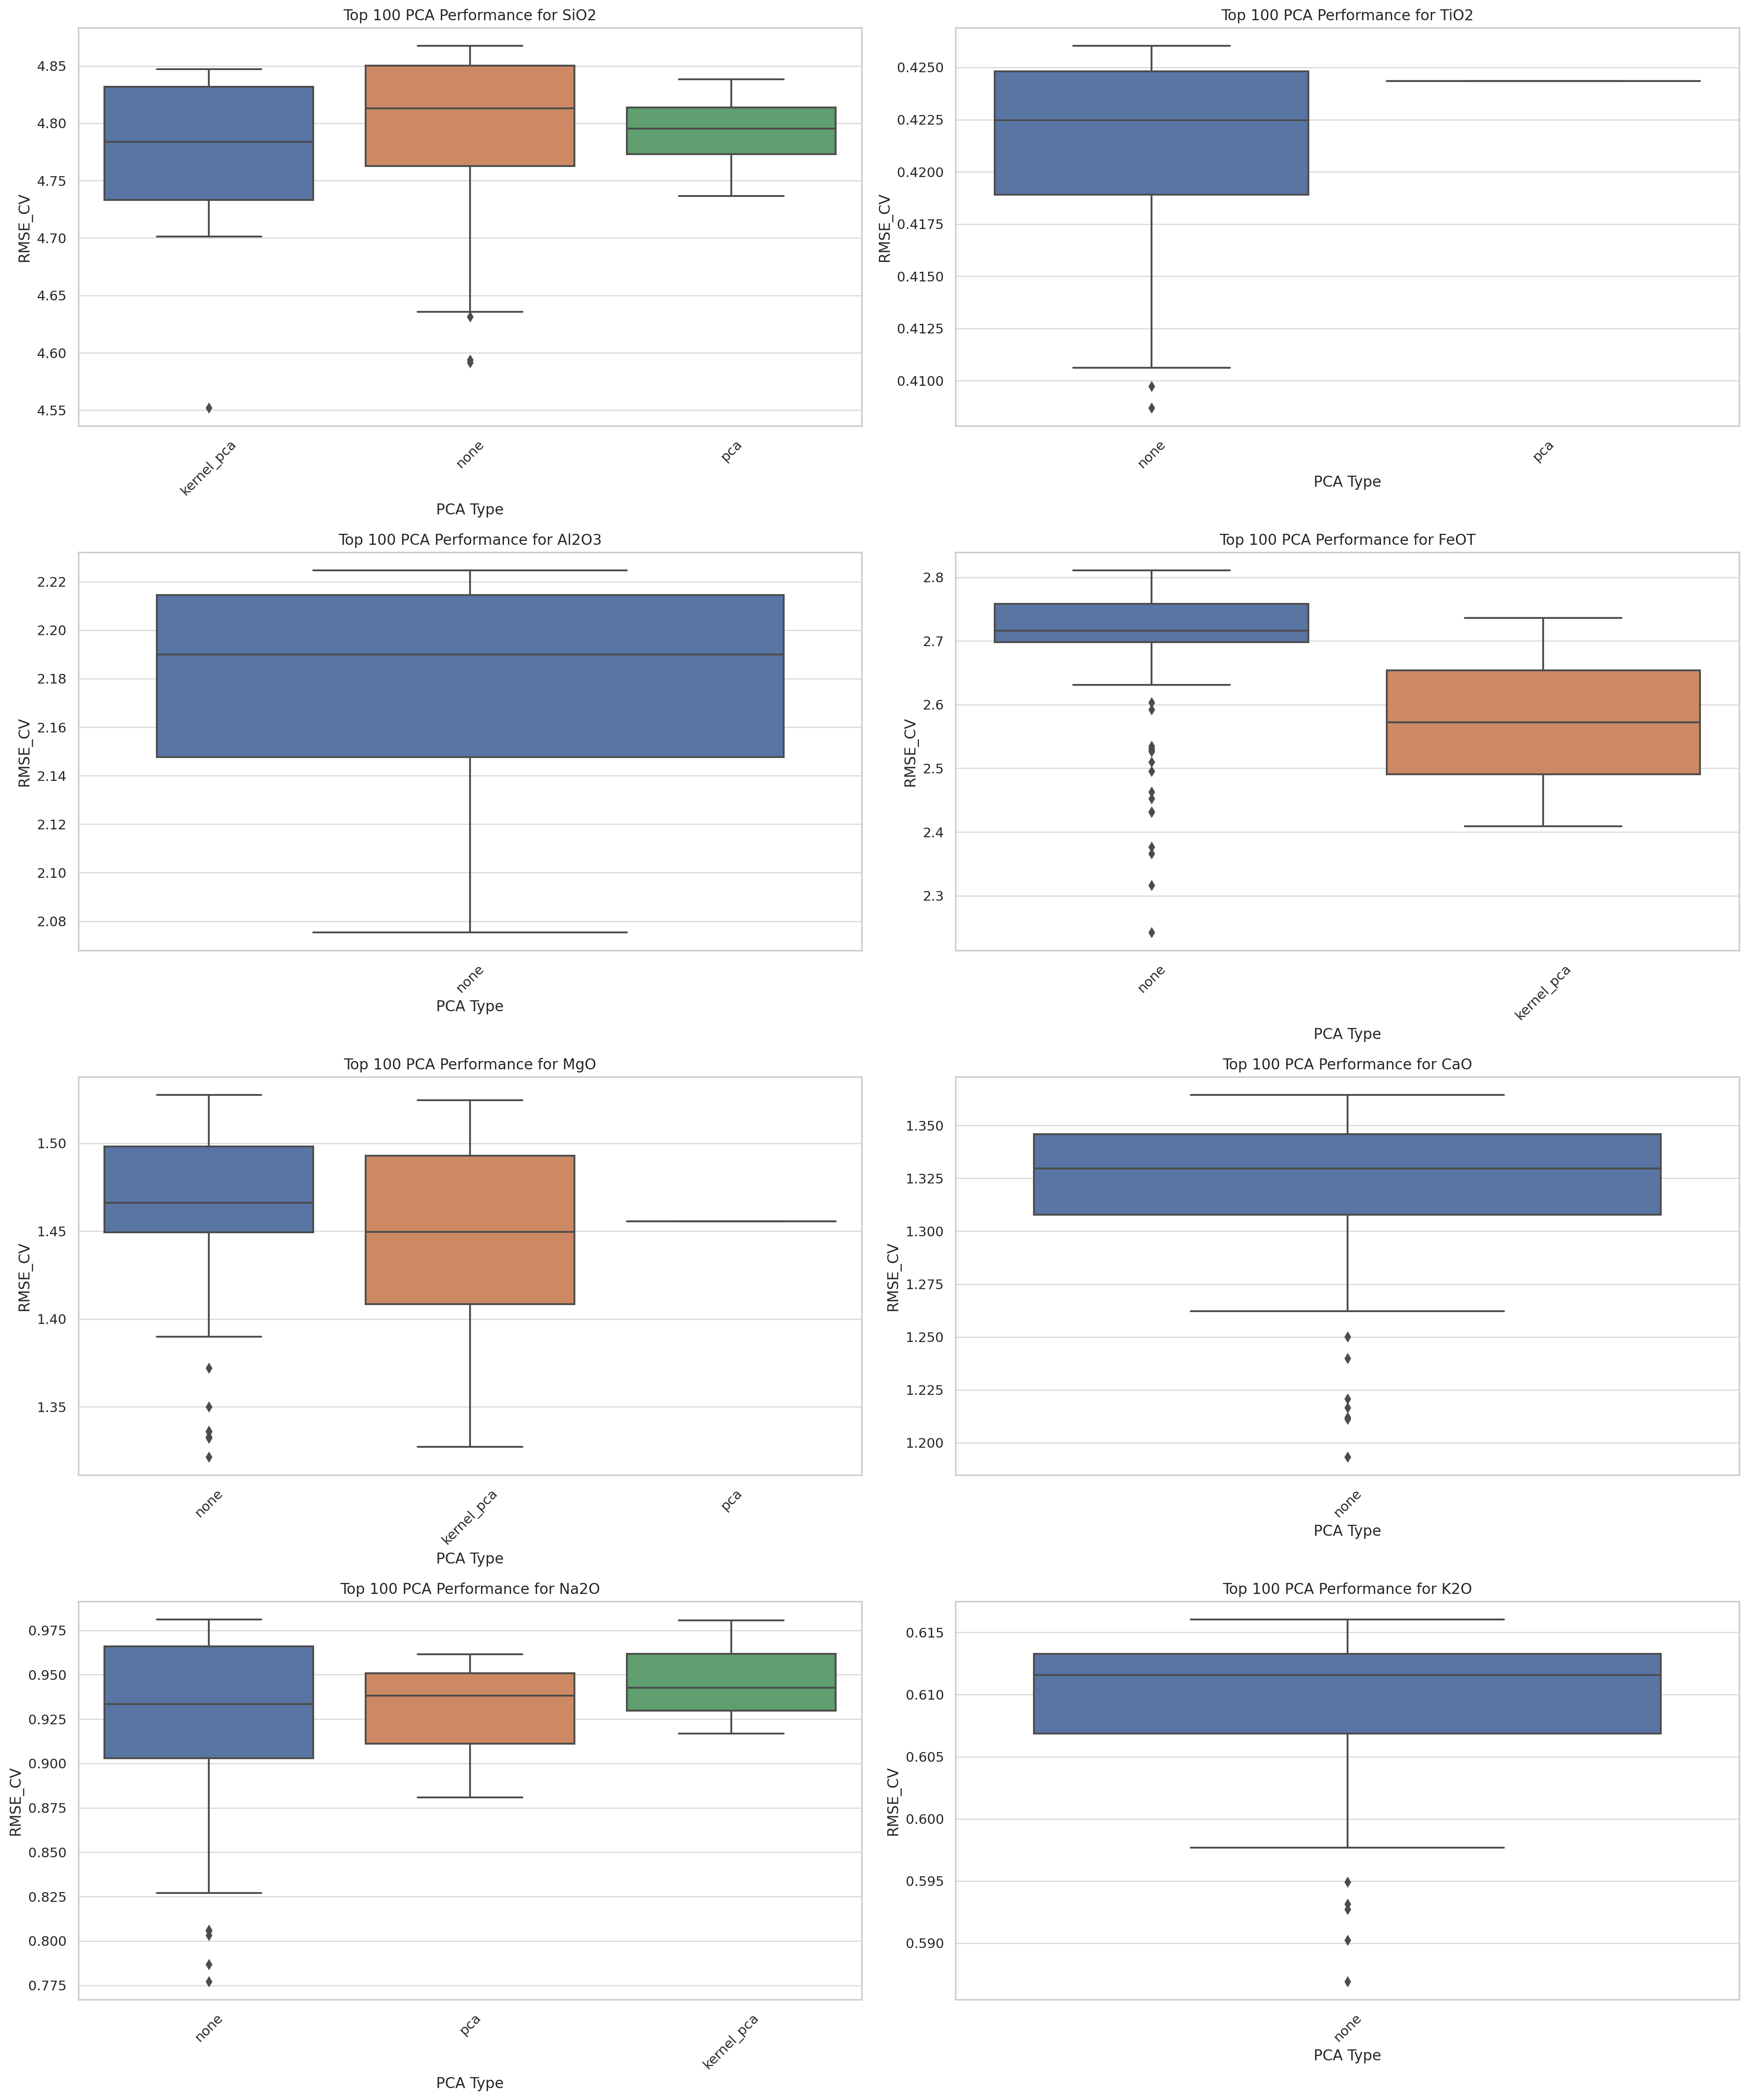
\includegraphics[width=\textwidth]{images/top100/pca.png}
    \caption{Top 100 \gls{pca} performance across oxides. The subplots present the distribution of \gls{rmsecv} values for the top 100 trials for each \gls{pca} type across the different oxides. This allows us to understand the impact of \gls{pca} techniques on model performance for each oxide within the top-performing trials.}
    \label{fig:top100_pca}
\end{figure*}


% - [ ] Show figures/tables showing how the various configuration elements fared
% - [x] Show table with Optuna model, preprocessor, etc., counts
% - [ ] Present best model configurations
% 	- Already have these in the appendix. May want to just include them in the main report.
% 	- Need to clarify in the text that they represent the single best performing configuration for each oxide as measured by RMSECV.

